\documentclass[10pt]{article}
\title{Lineaire optimalizatie [D0H42a] - Samenvatting\\*2011-2012}
\author{Wouter Schaekers\\*---\\*2/3Bach Informatica - 2Bach Handelsingenieur\\2Bach Handelsingenieur in de Beleidsinformatica\\Master Handelsingenieur in de Beleidsinformatica}
\usepackage{amsmath}
\usepackage{amssymb}
\usepackage{graphicx}
\usepackage[top=25mm, bottom=25mm, left=25mm, right=25mm]{geometry}
\usepackage{color}
\usepackage{multicol}
\usepackage{listings}
\usepackage{fancyhdr}
\definecolor{gray}{RGB}{145,145,145}
\definecolor{brown}{RGB}{139,69,19}
\definecolor{blue}{RGB}{0,0,255}
\definecolor{green}{RGB}{0,100,0}
\definecolor{red}{RGB}{255,0,0}
\pagestyle{fancy}
\begin{document}
\maketitle
\setcounter{section}{-1}
\setcounter{page}{0}
\renewcommand{\contentsname}{Inhoudstafel}
\setcounter{tocdepth}{3}
\tableofcontents
\clearpage
\section{Inleiding en inhoudstafel}
Deze samenvatting is gemaakt voor de studenten van 2/3Bach Informatica, 2Bach Handelsingenieur, 2Bach Handelsingenieur in de Beleidsinformatica en Master Handelsingenieur in de Beleidsinformatica.\\*
Deze samenvatting is gebaseerd op het boek. Hierbij is de negende, herziene uitgave van de cursus 'Lineair Optimaliseren' gebruikt.\\*
Deze samenvatting bevat voorbeelden die rechtstreeks uit de cursus komen. Deze voorbeelden vallen onder de copyright van de auteurs van de cursus (D. Goossens en F.C.R. Spieksma).\\*
Deze samenvatting is hoogstwaarschijnlijk niet foutloos. Eventuele aanpassingen kunnen gemaakt worden op https://github.com/WouterSchaekers/LineaireOptimalisatie-Samenvatting.\\*
De auteur is niet bereid samenvattingen te signeren.\\*
Het sturen van spam is verboden. Het stalken van de auteur is, na toestemming, slechts in uitzonderlijke omstandigheden toegestaan.\\*
De auteur is niet verantwoordelijk voor enige gevolgen van het gebruik van deze bundel.\\*
Het is verboden de afgedrukte versie van de samenvatting te verbranden of op te eten.\\*\\*
Geen langdurig gebruik zonder wiskundig advies. Alle lijnstukken voorbehouden.\\\\
This resume is released under the beerware license. Donations on the following bitcoin address are really appreciated. Thanks.\\\\\\\\\\\\\\\\\\\\\\\\\\\\\\\\\\\\\\\\\\
\begin{center}
\textit{"Alles moet zo eenvoudig mogelijk gemaakt worden, maar niet eenvoudiger dan dat."}\\*-\\*Albert Einstein
\end{center}
\begin{center}

\includegraphics[scale=0.5]{BitcoinAddress.png}\\*

\includegraphics[scale=0.02]{Bitcoin.png} \textbf{1HgMRMvafHHFPzhn6Nwzjp6gVb5Qzrnn4r}
\end{center}
\clearpage
\section{Inleiding}
Niet belangrijk. Slaan we over.
\section{Het formuleren van lineaire optimaliseringsmodellen}
In de economie is het vaak belangrijk om iets te maximaliseren (winst) of iets te minimaliseren (kosten). Om tot een maximale winst of minimale kost te komen, kunnen we gebruik maken van lineaire optimaliseringsmodellen. Zulk een optimaliseringsmodel is in feite niets anders dan een wiskundig model waarin opgelegd wordt om iets te maximaliseren of minimaliseren, waarbij aan bepaalde constraints moet worden voldaan.
\subsection{Een eerste voorbeeld}
Het is het best om dit te illustreren met het voorbeeld 2.1:\\*\\*
\textit{Een bedrijf vervaardigt houten deuren en houten tafelbladen. Per houten deur moet 1 uur aan houtbewerking en 2 uur aan afwerking (schuren en schilderen) besteed worden. Voor elk tafelblad is 1 uur houtbewerking en 1 uur afwerking nodig. Per week kunnen 80 werkuren besteed worden aan houtbewerking en 100 aan afwerking. De grondstoffen zijn onbeperkt voorradig. Uit het verleden is gebleken dat per week maximaal 40 deuren verkocht kunnen worden. Het bedrijf kan de deuren en de tafelbladen verkopen met een winst van respectievelijk 300 Eurocent en 200 Eurocent per stuk. Hoe kunnen we de wekelijkse winst zo groot mogelijk maken?}\\\\
Dit vraagstuk bevat 2 variabelen, namelijk het aantal geproduceerde deuren en het aantal geproduceerde tafelbladen. Deze gaan we in ons model voorstellen door respectievelijk $x_1$ en $x_2$.\\*
Het overeenkomstig optimaliseringsmodel:\\*
maximaliseer $z = 300x_1 + 200x_2$\\*
\textit{Dit is de winst die gemaximaliseerd moet worden. Dit wordt ook wel de doelfunctie genoemd.}\\*
zodanig dat\\*
$2x_1 + x_2 \le 100$\\*
\textit{Het maximaal aantal uren dat kan besteed worden aan afwerking.}\\*
$x_1 + x_2 \le 80$\\*
\textit{Het maximaal aantal uren dat kan besteed worden aan houtbewerking.}\\*
$x_1 \le 40$\\*
\textit{Er kunnen maximaal 40 deuren per week verkocht worden.}\\*
$x_i \ge 0$\\*
\textit{Dit is een beperking die er zo goed als altijd bij moet. Een negatieve hoeveelheid producten produceren is wiskundig heel leuk, maar in de realiteit niet echt haalbaar.}\\\\
In dit hoofdstuk wordt er nog niet ingegaan op hoe dat zulke modellen opgelost moeten worden. Dat is pas voor hoofdstuk 5.\\*
Voor een extra voorbeeld (2.2), zie de cursus.
\subsection{Lineariteit}
Deze cursus gaat over "lineaire optimaliseringsproblemen" of "LO problemen". Het spreekt voor zich dat er enkel lineaire functies of ongelijkheden gebruikt worden. Uitdrukkingen zoals $x_1^2$, $x_1x_2$ of $\sqrt{x_1}$ mogen niet voorkomen.\\*
De laatste regel van een LO model bevat de tekenbeperking van de variabelen. Deze kunnen positief ($ge$), negatief ($le$) of onbepaald ($o.i.t.$ (onbeperkt in teken)) zijn.
\subsection{Toepasbaarheid van lineaire modellen}
\textbf{Proportionaliteit}: De winst bij het produceren van twee eenheden moet twee keer zo groot zijn als de winst bij het produceren van \'e\'en eenheid.\\*
\textbf{Additiviteit}: De winst bij het produceren van \'e\'en eenheid van product 1 blijft hetzelfde, ongeacht of dat er van product 2 \'e\'en eenheid of twee eenheden geproduceerd worden.\\*
\textbf{Deelbaarheid}: De oplossing $\in \mathbb{Z}$.\\\\
Er zijn situaties waarbij de proportionaliteit of de additiviteit kan geschonden worden. Bijvoorbeeld bij schaalvoordelen, steup kosten en interactie tussen verschillende producten.
\section{Voorbeelden}
Dit hoofdstuk behandelt de vele verschillende vormen van optimaliseringsmodellen. Deze worden uitvoerig beschreven in de cursus, maar dit is mijns inziens niet nuttig. Het enige wat je nodig hebt om zulke modellen op te stellen is gezond verstand. Voor de volledigheid overlopen we toch alle modellen die besproken worden en vatten het belangrijkste samen. Voor de voorbeelden zelf, zul je de cursus moeten raadplegen.
\subsection{Investeringsprobleem}
Om toch een algemeen idee te krijgen maken we voor dit probleem een uitzondering en plaasten we wel een voorbeeld in de samenvatting.\\
Een investeringsprobleem gaat over twee of meersdere projecten waarin ge\"investeerd kan worden. Het is de bedoeling om de winst te maximaliseren door voor elk van deze projecten een deel geld te investeren.\\*
Gegeven is de hoeveelheid winst en verlies per tijdstip per project. Het aandeel waarin ge\"investeerd wordt in een bepaald project, blijft constant over de tijd. Meestal is het zo dat op het geld dat na een tijdstip overschiet rente kan worden vergaard (in ons voorbeeld $2\%$) en op het bedrag dat geleend wordt rente moet worden betaald (in ons voorbeeld $2.5\%$).\\*
De beslissingsvariablen zijn dus de fracties van de projecten (in ons voorgesteld door $p_i$).\\*
Andere variabelen zijn het geleend bedrag per tijdstip ($b_i$) en het gespaarde bedrag per tijdstip ($s_i$).\\\\
Het (vereenvoudigd) voorbeeld:
\begin{table}[!h]
\begin{center}
\begin{tabular}{| c | c | c |} \hline
Tijdstip & Project 1 & Project 2\\ \hline
1 & +1 & -1 \\ \hline
2 & -2 & +2 \\ \hline
3 & +3 & -3 \\ \hline
\end{tabular}
\end{center}
\end{table}
\\*
Zoals uit de bovenstaande tabel kan worden afgeleid, is het niet nuttig om te investeren in project 2. Maar dat is irrelevant voor het opstellen van het model.\\*
Voor elk tijdstip beschikken we over 1 euro, die we niet moeten teruggeven. Bij het begin beschikken we dus over $1+b_1$ euro. Een vereiste is dat we niet in het rood gaan. We mogen niet meer uitgeven dan we hebben (inclusief het geleende bedrag). Hieruit volgt de eerste constraint:\\*
$p_2-p_1 \le 1+b_1$\\*
Het gespaarde bedrag komt overeen met:\\*
$s_1 = 1+b_1+p_1-p_2$\\
Bij de volgende constraint moeten we het gespaarde en het geleende bedrag van het vorige tijdstip in rekening brengen. Bovendien legt de opgave ons op dat we niet meer dan 1 euro per tijdstip mogen lenen. Dit levert ons het volgende model op:\\
max $z = s_3$\\*
zdd\\*
$s_1-(b_1+p_1-p_2) = 1$\\*
$s_2-(b_2-2p_1+2p_2+1.02s_1-1.025b_1) = 1$\\*
$s_3-(b_3+3p_1-3p_2+1.02s_2-1.025b_2) = 1$\\*
$0 \le p_i \le 1$ voor $i = 1,2$\\*
$0 \le b_i \le 1$ voor $i = 1,2$\\*
$0 \le s_i$ voor $i = 1\dots3$
\subsection{Mengprobleem}
Hier gaat het over het algemeen over een aantal types van producten die door het mengen van een aantal andere (basis)producten tot stand komt. (In de cursus staat een voorbeeld over drie types benzine die tot stand komen door drie soorten ruwe olie te mengen.) Voor het mengen van de (basis)producten bestaan regels. Zo moet elk type aan bepaalde voorwaarden voldoen. (Bijvoorbeeld een bepaald octaangehalte dat gehaald moet worden.) Dit soort van problemen is over het algemeen een stuk makkelijker dan het vorige probleem omdat de constrains hier bijna letterlijk in de opgave staan.\\*
De beslissingsvariabelen zijn het aantal basisproducten dat je nodig hebt voor elk type van producten te kunnen produceren.
\subsection{Menuprobleem}
Het samenstellen van een 'dieet' dat aan voorwaarden voldoet (hoeveelheid calcium, vitamines, \dots). De beslissingsvariabelen zijn simpelweg de hoeveelheid van elk product. Het kan zijn dat er een hulpvariabele nodig is (zoals de dagelijkse hoeveelheid energie, die tussen twee waarden moet liggen). Dit probleem is nog makkelijker dan het mengprobleem.
\subsection{Roosterprobleem}
Elke dag heeft men een verschillend aantal werknemers nodig. Elke werknemer werkt een x aantal opeenvolgende dagen. De bedoeling is om zo weinig mogelijk werknemers in dienst te hebben, zodat de kosten zo laag mogelijk zijn.
\subsection{Stroomprobleem}
Een aantal basisproducten kan worden herwerkt tot meerdere producten. Deze producten kunnen dan nog eens verder verwerkt worden. Dit probleem kan in combinatie voorkomen met een mengprobleem.
\subsection{Productie-voorraadprobleem}
Een bedrijf kan een maximaal aantal boten produceren per kwartaal. Dat bedrijf kan dit maximaal aantal overschrijden door zijn arbeiders overuren te laten draaien. Uiteraard is het zo dat overuren meer kosten. Het bedrijf kan ook beslissen om meer te produceren dan de vraag in dat kwartaal om zo zijn werknemers geen overuren te laten draaien. Het probleem is dat de opslag van deze goederen ook geld kost.\\*
De beslissingsvariabelen zijn hier het aantal producten gemaakt tijdens de normale werkuren, het aantal producten gemaakt tijdens de overuren en de voorraad in elk kwartaal.
\subsection{Versnijdingsprobleem}
Een bedrijf heeft rollen van een bepaalde breedte. Een klant wil $x$ rollen met een bepaalde breedte en $y$ rollen met een andere breedte.\\*
Dit probleem kan opgelost worden door op te schrijven op welke manieren de 'hoofdrol' kan versneden worden in de rollen die de klant nodig heeft. Daarna is het slechts een kwestie van het model juist op te stellen.\\\\
Bijvoorbeeld:\\*
Hoofdrol = 2 meter\\*
Benodigde rollen = 1 meter en 0.5 meter\\*
Patronen:\\*
$P_1 = 2x1$\\*
$P_2 = 1x1\ 2x0.5$\\*
$P_3 = 4x0.5$
\subsection{Netwerkproblemen}
\subsubsection{Transportproblemen}
Een bedrijf heeft een aantal vestigingen en een aantal verdeelcentra in verschillende steden. Elk verdeelcentrum heeft een verschillende vraag. Elke vestiging heeft een verschillende productie. Het is de bedoeling om zo weinig mogelijk afstand af te leggen door aan de vraag te kunnen voldoen.\\*
De beslissingsvariabelen zijn het aantal producten dat op elke lijn wordt getransporteerd.
\subsubsection{Toewijzigingsprobleem}
Een bedrijf heeft een aantal mensen in dienst. Elk van deze mensen is goed in een bepaalde sectie. Het is de bedoeling om elk van deze mensen toe te wijzen aan exact \'e\'en van deze secties (en dus niet meer), zodat het bedrijf als geheel het beste presteert. (Let op, de voorwaarde 'exact \'e\'en' zijn heel veel constraints!) Het is onmogelijk dat er tijdens de uitvoer van een sectie gewisseld wordt. Elke persoon doet zijn sectie volledig uit.
\subsubsection{Distributieprobleem}
Dit is in feite hetzelfde als het transportprobleem. Het enige verschil is dat het transport niet meer rechtstreeks gaat, maar met tussenstops. De tussenstops kunnen met elkaar in verbinding staan, waardoor het soort van grafenprobleem wordt. De oplossing is niet moeilijk. Stel voor elk distributiepunt dat het aantal producten dat toekomt gelijk moet zijn aan het aantal producten dat er vertrekt.
\section{De geometrie van LO-problemen}
Dit hoofdstuk probeert de lezer inzicht te geven in LO-problemen door middel van grafische technieken.
\subsection{Grafisch oplossen van LO-problemen met twee variabelen}
Wanneer een probleem slechts twee variabelen heeft, kan elke oplossing worden aangeduid in het vlak. Ook elke constraint kan worden voorgesteld door een rechte in datzelfde vlak.\\\\
We beschouwen het volgende voorbeeld:\\*
max $z = 300x_1 + 200x_2$\\*
zdd\\*
$2x_1 + x_2 \le 100$\\*
$x_1 + x_2 \le 80$\\*
$x_1 \le 40$\\*
$x_i \ge 0$ voor $i = 1,2$\\*
Dit levert het volgende toegelaten gebied op:\\*
\begin{center}
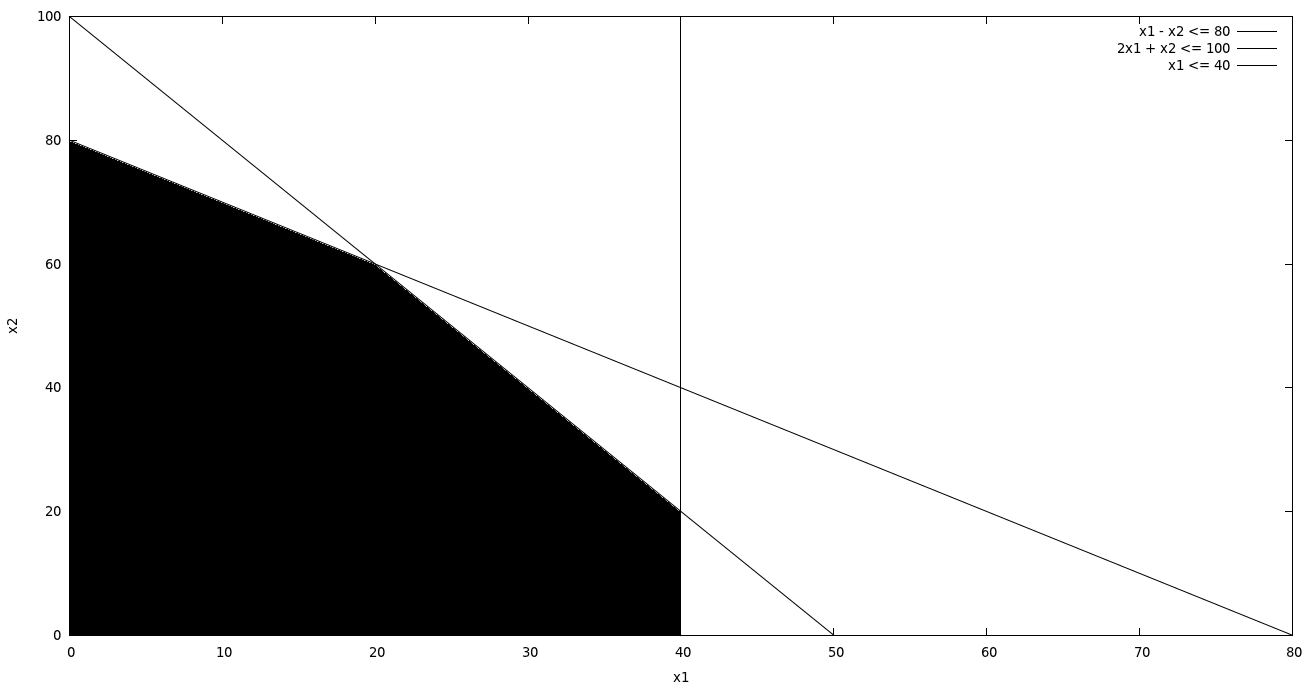
\includegraphics[width = 130mm]{geometrie1.png}
\end{center}
%gnuplot> set xlabel "x1"
%gnuplot> set ylabel "x2"
%gnuplot> plot "data.dat" using 1:2 title 'x1 - x2 <= 80' with lines lt -1, "data.dat" using 3:4 title '2x1 + x2 <= 100' with lines lt -1, "data.dat" using 5:6 title 'x1 <= 40' with lines lt -1
Enkel de doelfunctie moet nog gevisualiseerd worden. Het probleem is dat $z$ geen constantie is en gemaximaliseerd moet worden. Daarom moeten we gewoon een $x_1$ en $x_2$ kiezen uit het toegelaten gebied en invullen in de vergelijking. Laten we $(20, 0)$ kiezen. Dit levert $z = 6000$ op. Nu kunnen we $300x_1 + 200x_2 = 6000$ ook tekenen op de grafiek (deze lijn wordt ook wel een isokostlijn of een isowinstlijn genoemd).\\*
Nu, 6000 is niet de maximale waarde die $z$ kan aannemen. Daarom zullen we de lijn evenwijdig verschuiven naar rechtsboven tot we de rand hebben bereikt van het toegelaten gebied:\\*
\begin{center}
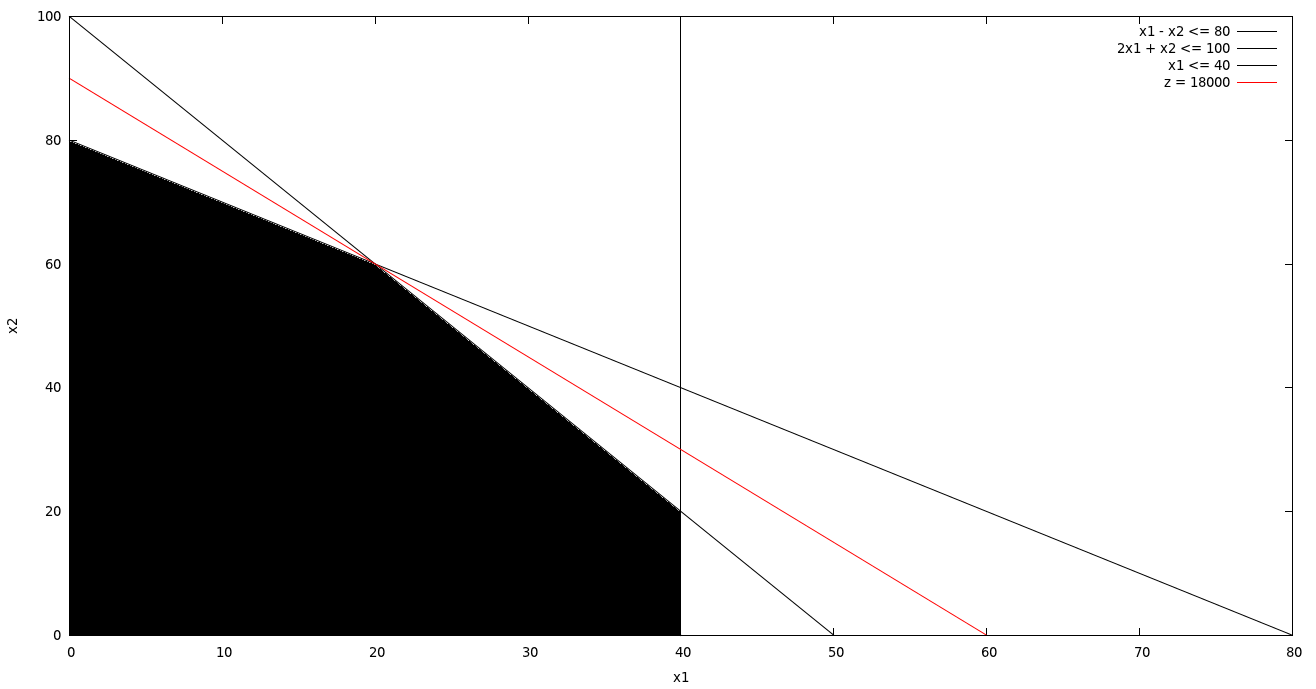
\includegraphics[width = 130mm]{geometrie2.png}
\end{center}
%gnuplot> set xlabel "x1"
%gnuplot> set ylabel "x2"
%gnuplot> plot "data.dat" using 1:2 title 'x1 - x2 <= 80' with lines lt -1, "data.dat" using 3:4 title '2x1 + x2 <= 100' with lines lt -1, "data.dat" using 5:6 title 'x1 <= 40' with lines lt -1, "data.dat" using 7:8 title 'z = 18000' with lines lt 1
Het spreekt voor zich dat deze techniek ook werkt op een minimalisatieprobleem.
\subsection{Bijzondere situaties}
\subsubsection{Meerdere oplossingen}
Het is perfect mogelijk dat eer meerdere optimale oplossingen voorkomen. Dit kan gebeuren wanneer de doelfunctie-lijn evenwijdig ligt aan een grenslijn.
\subsubsection{Geen toelaatbare oplossingen}
Dit kan voorkomen wanneer de voorwaarden te strikt zijn.
\subsubsection{Onbegrensde oplossing}
Dit kan voorkomen wanneer er niet genoeg voorwaarden zijn.
\subsection{Definities, terminologie en eigenschappen}
\textbf{Bindende beperking}: Een beperking waarbij, na substitutie van de optimale oplossing, het linker en rechterdeel van de vergelijking aan elkaar gelijk zijn. Bij een niet-bindende beperking is dit uiteraard niet zo.\\*
\textbf{Redundante beperking}: Een beperking die niet nodig is om tot dezelfde oplossing te komen.\\\\
Enkele eigenschappen:\\*
Het toegelaten gebied van een LO-probleem is een convexe verzameling.\\*
Het toegelaten gebied van een LO-probleem bevat een eindig aantal extreme punten (= punten in een convexe verzameling waarvoor geldt dat, voor elk lijnstuk dat volledig in deze verzameling ligt en dit punt bevat, dit punt een eindpunt is van dit lijnstuk).\\*
Indien het LO-probleem een optimale oplossing heeft, dan bestaat er tenminste \'e\'en extreem punt dat optimaal is.\\
Het is makkelijk in te zien dat deze eigenschappen juist zijn. De bewijzen van deze eigenschappen worden in deze cursus achterwege gelaten.\\\\
PS: De optimale oplossing (als er \'e\'en bestaat) kan dus altijd gevonden worden door de extreme punten af te lopen.
\section{De simplex methode - deel 1}
Dit hoofdstuk behandelt de simplex methode, een methode om lineaire optimaliseringsproblemen op te lossen.\\*
De simplex methode vereist dat het LO-probleem in de standaardvorm staat. De standaardvorm is van de vorm:\\*
maximaliseer $\sum_{j=1}^nc_jx_j$\\*
zdd $\sum_{j=1}^na_{ij}x_j \le b_i$ voor $i = 1 \dots m$\\*
$x_j \ge 0$ voor $j = 1 \dots n$\\\\
Elk probleem zal dus eerst moeten omgezet worden naar de standaardvorm:
\begin{itemize}
\item minimaliseren van $f(x)$ = maximaliseren van $-f(x)$
\item $\sum_{j=1}^na_{ij}x_j \ge b_i$ = $-\sum_{j=1}^na_{ij}x_j \le -b_i$
\item $\sum_{j=1}^na_{ij}x_j = b_i$ = ($\sum_{j=1}^na_{ij}x_j \le b_i$ $\&$ $-\sum_{j=1}^na_{ij}x_j \le -b_i$)
\item $x$ is oit $\Rightarrow$ introduceer $x^+$ en $x^-$; $x^+, x^- \ge 0$ en vervang $x$ door $x^+ - x^-$
\end{itemize}
\subsection{Een voorbeeld}
We volgen het voorbeeld uit de cursus.\\
Maximaliseer $5x_1 + 4x_2 + 3x_3$\\*
Zodanig dat\\*
$2x_ 1 + 3x_ 2 + x_3 \le 5$\\*
$4x_1 + x_2 + 2x_3 \le 11$\\*
$3x_1 + 4x_2 + 2x_3 \le 8$\\*
$x_i \ge 0$ voor $i = 1\dots3$\\
De opgave staat al in standaardvorm.\\\\
De eerste stap van de simplex methode bestaat erin spelingsvariabelen te introduceren.\\*
Laten we kijken naar de eerste regel: $2x_1 + 3x_ 2 + x_3 \le 5$. Voor elke oplossing geldt dat het linkerdeel kleiner of gelijk is aan 5. Het verschil tussen het linkerdeel en het rechterdeel heet de 'speling'. We defini\"eren $x_4 = 5 - (2x_1 + 3x_ 2 + x_3)$ , $x_4 \ge 0$ als deze speling. De opgave kan herschreven worden in functie van de spelingswaarden:\\
Maximaliseer $5x_1 + 4x_2 + 3x_3$\\*
Zodanig dat\\*
$x_4 = 5 - (2x_ 1 + 3x_ 2 + x_3)$\\*
$x_5 = 11 - (4x_1 + x_2 + 2x_3)$\\*
$x_6 = 8 - (3x_1 + 4x_2 + 2x_3)$\\*
$x_i \ge 0$ voor $i = 1\dots6$\\\\
Het idee van de simplex methode is om telkens een betere oplossing te vinden. In ons voorbeeld starten we met $x_i = 0$ voor $i = 1\dots3$. $z$ is dan $0$. We laten $x_2 = x_3 = 0$ en hogen $x_1$ op. $x_1$ kan de waarde $2.5$ bereiken (niet $3$, want dan worden de spelingsvariabelen negatief). Hoe kunnen we dat weten? De voorwaarde $x_4 = 5 - (2x_1 + 3x_ 2 + x_3) \ge 0$ impliceert dat $x_1 \le \frac{5}{2}$ ($x_5 \ge 0$ impliceert $x_1 \le \frac{11}{4}$ en $x_6 \ge 0$ impliceert $x_1 \le \frac{8}{3}$).\\*
Dus we vinden de voorlopige oplossing $z = 25/2$. Merk op dat $x_4 = 0$.\\*
Om verder te kunnen werken, moeten alle variabelen die $0$ zijn geworden naar rechts verhuizen. Dit kan door $x_1$ te substitueren in alle vergelijkingen. We krijgen:\\*
$z = \frac{25}{2} - \frac{7}{2}x_2 + \frac{1}{2}x_3 - \frac{5}{2}x_4$\\*
$x_1 = \frac{5}{2} - \frac{3}{2}x_2 - \frac{1}{2}x_3 - \frac{1}{2}x_4$\\*
$x_5 = 1 + 5x_2 + 2x_4$\\*
$x_6 = \frac{1}{2} + \frac{1}{2}x_2 - \frac{1}{2}x_3 + \frac{3}{2}x_4$\\*
Merk op dat de vergelijking van $x_1$ is toegevoegd en de vergelijking van $x_4$ is weggevallen (deze was toch $x_4 = 0$).\\*
We proberen de waarde van $z$ verder op te hogen. Dit kan enkel door $x_3$ op te hogen. De maximale waarde voor $x_3$ is $1$, aangezien $x_i \ge 0$. De vergelijking voor $x_3 = 1 + x_2 + 3x_4 - 2x_6$.\\
Het nieuwe stelsel:\\*
$z = 13 - 3x_2 - x_4 - x_6$\\*
$x_1 = 2 - 2x_2 - 2x_4 + x_6$\\*
$x_3 = 1 + x_2 + 3x_4 - 2x_6$\\*
$x_5 = 1 + 5x_2 + 2x_4$\\
We hebben de oplossing gevonden. $z = 13$, aangezien $x_i \ge 0$. De waarden van de andere variabelen zijn onmiddellijk af te lezen. Merk op dat $x_5 = 1$. Deze variabele was de spelingsvariabele. Als we $x_1 = 2, x_2 = 0\ en\ x_3 = 1$ invullen in vergelijking $4x_1 + x_2 + 2x_3 \le 11$, dan krijgen we $10 \le 11$. De speling is inderdaad $1$.
\subsection{Dictionairs}
De bovenstaande oplossingsmethode kan ook algemeen opgesteld worden. De opdracht is als volgt:\\*
Maximaliseer $\sum_{j=1}^nc_jx_j$\\*
Zodanig dat $\sum_{j=1}^na_{ij}x_j \le b_i$\\*
$x_j \ge 0$ voor $i = 1 \dots m, j = 1 \dots n$\\\\
Dit vormen we om naar:\\*
$z = \sum_{j=1}^nc_jx_j$\\*
$x_{n+i} = b_i - \sum_{j=1}^na_{ij}x_j$ voor $i = 1 \dots m,\ j = 1 \dots n$\\*\\*
Bovenstaand stelsel wordt een dictionair genoemd, omdat de waarden die gezogd worden onmiddellijk af te lezen zijn uit de vergelijkingen.\\*
Wanneer we de waarde $0$ kiezen voor de variabelen aan de rechterkant, dan vinden we een toelaatbare oplossing (wat logisch is, want het is dan rechtstreeks een oplossing van het stelsel). Dictionairs die deze eigenschap bezitten, heten toelaatbare dictionairs. Merk op dat niet alle toelaatbare oplossingen kunnen worden voorgesteld worden met een toelaatbare dictionair. Zo kan de toelaatbare oplossing $x_1 = 1, x_2 = 0, x_3 = 1, x_4 = 2, x_5 = 5, x_6 = 3$ niet voorgesteld worden door een toelaatbare dictionair.\\*
Oplossingen die beschreven worden met een dictionair worden basisoplossingen genoemd. Van zodra een basisoplossing een variabele heeft met een waarde die strikt kleiner is dan $0$, dan spreken we over een ontoelaatbare basisoplossing.\\\\
Variabelen aan de linkerkant van de dictionair heten basisvariabelen, de variabelen aan de rechterkant heten niet-basisvariabelen. De basisvariabelen vormen de basis. De vergelijking die de sterkste beperking oplegt en dus omgevormd moet worden (om te substitueren in de andere vergelijkingen), heet de spilrij.\\\\
Verder vermelt de cursus dat de volgorde van de vergelijkingen in een dictionair niet worden gesorteerd volgens de index van de basisvariablen om zo 'de relatie tussen de dictionair en het oorspronkelijke model te behouden'. Dit is een heel mooie filosofie, maar aan zulke futuliteiten zullen we geen tijd verspillen.
\section{De simplex methode - deel 2}
In het vorige hoofdstuk hebben we de simplex methode behandeld. Dit hoofdstuk behandelt de vraag of de simplex methode wel altijd kan worden toegepast.
\subsection{Iteratie}
Kunnen we vastlopen in een iteratie?\\*
Voor deze stap moeten we een inkomende variabele selecteren een een uitgaande variabele vinden.\\*
De inkomende variabele is een niet-basisvariabele met een positieve co\"effici\"ent op de eerste rij van de dictionair (de doelfunctie). Indien er geen positieve co\"effici\"enten te vinden zijn, dan is de dictionair optimaal. Bij meerdere mogelijkheden, maakt het niet uit welke inkomende variabele gekozen wordt.\\
De uitgaande variabele is de basisvariabele waarvan de overeenkomstige vergelijking de meest strikte bovengrens oplegt aan de stijging van de inkomde variabele. Ook hier kunnen er veel of geen te vinden zijn. In het eerste geval moet je er gewoon \'e\'en kiezen. In het tweede geval is er geen bovengrens en is de oplossing dus onbegrensd.
\subsection{Gedegenereerdheid}
Wanneer meerdere variabelen de basis kunnen verlaten, heeft dat een aantal consequenties. Beschouw het volgende voorbeeld:\\*
$z = 2x_1 - x_2 + 8x_3$\\*
$x_4 = 1 - 2x_3$\\*
$x_5 = 3 - 2x_1 + 4x_2 - 6x_3$\\*
$x_6 = 2 + x_1 - 3x_2 - 4x_3$\\
De meest strikte beperking voor $x_3$ is $1/2$. Dit geldt voor alle vergelijkingen. We kiezen de vergelijking van $x_4$ als de spilrij. Substitutie geeft ons:\\*
$z = 4 + 2x_1 - x_2 - 4x_4$\\*
$x_3 = \frac{1}{2} - \frac{1}{2}x_4$\\*
$x_5 = -2x_1 + 4x_2 + 3x_4$\\*
$x_6 = x_1 - 3x_2 + 2x_4$\\\\
De basisvariabelen $x_5$ en $x_6$ hebben waarde $0$.\\*
In de volgende stap van de iteratie is $x_1$ de inkomende variabele en $x_5$ de uitgaande variabele. $x_1$ is in dit geval $0$. $z$ blijft dus onveranderd, de dictionair is gedegenereerd. Dit verschijnsel kan een aantal keer voorkomen, maar is onschuldig. De volgende iteratie is weer gedegenereerd. De iteratie daarna is niet gedegenereerd (en optimaal).\\\\
Het is weliswaar mogelijk dat we er nooit uitgeraken en dat we blijven itereren zonder dat de waarde van $z$ verhoogt. Na verloop van tijd zullen we dan opnieuw dezelfde dictionair tegenkomen. Dit heet cykelen.
\subsection{Begin}
Kunnen we wel beginnen met de simplex methode?\\*
De simplex methode begint normaliter met:\\*
$z = \sum_{j=1}^nc_jx_j$\\*
$x_{n+i} = b_i - \sum_{j=1}^na_{ij}x_j$ voor $i = 1 \dots m,\ j = 1 \dots n$\\
De voorwaarde van dit stelsel is dat $b_i$ allen positief zijn (anders is de oorsprong geen toelaatbare oplossing). Het kan perfect voorkomen dat dit niet zo is. Een voorbeeld:\\\\
Maximaliseer $x_1 - x_2 + x_3$\\*
zodanig dat\\*
$2x_1 - x_2 + 2x_3 \le 4$\\*
$2x_1 - 3x_2 + x_3 \le -5$\\*
$-x_1 + x_2 - 2x_3 \le -1$\\*
$x_i \ge 0$ voor $i = 1\dots3$\\\\
De oplossing is eenvoudig. Introduceer een extra variabele $x_0$ en vorm het stelsel om naar:\\\\
$w = -x_0$\\*
$x_4 = 4 - (2x_1 - x_2 + 2x_3 - x_0)$\\*
$x_5 = -5 - (2x_1 - 3x_2 + x_3 - x_0)$\\*
$x_6 = -1 - (-x_1 + x_2 - 2x_3 - x_0)$\\\\
De bedoeling van dit hulpprobleem is om $w$ te maximaliseren. Ingaand = $x_0$ en uitgaand = $x_5$ geeft:\\\\
$w = -5 - 2x_1 + 3x_2 - x_3 - x_5$\\*
$x_4 = 9 - 2x_2 - x_3 + x_5$\\*
$x_0 = 5 + 2x_1 - 3x_2 + x_3 + x_5$\\*
$x_6 = 4 + 3x_1 - 4x_2 + 3x_3 + x_5$\\\\
We hebben $x_5$ gekozen als uitgaande variabele, omdat deze de kleinste $b$-waarde bevat. (Indien we bijvoorbeeld $x_6$ hadden gekozen als uitgaande variabele, dan was $x_5$ nog steeds negatief.)\\*
De laatste dictionair van het sub-probleem:\\\\
$w = -x_0$\\*
$x_4 = 3 - x_1 - x_6 + 2x_0$\\*
$x_3 = \frac{8}{5} - \frac{1}{5}x_1 + \frac{1}{5}x_5 + \frac{3}{5}x_6 - \frac{4}{5}x_0$\\*
$x_2 = \frac{11}{5} + \frac{3}{5}x_1 - \frac{2}{5}x_5 + \frac{1}{5}x_6 - \frac{3}{5}x_0$\\\\
Het hulpprobleem is opgelost. Om dit stelsel om te vormen tot het oorspronkelijke probleem, moet je gewoon $x_0$ negeren. De doelfunctie is terug de oorspronkelijke doelfunctie. Merk op dat er basisvariabelen in de doelfunctie kunnen zitten. Deze moeten eruit. Gebruik hiervoor substitutie:\\\\
$z = x_1 - (\frac{11}{5} + \frac{3}{5}x_1 - \frac{2}{5}x_5 + \frac{1}{5}x_6) + (\frac{8}{5} - \frac{1}{5}x_1 + \frac{1}{5}x_5 + \frac{3}{5}x_6)$\\\\
$z = -\frac{3}{5} + \frac{1}{5}x_1 - \frac{1}{5}x_5 + \frac{2}{5}x_6$\\*
$x_4 = 3 - x_1 - x_6$\\*
$x_3 = \frac{8}{5} - \frac{1}{5}x_1 + \frac{1}{5}x_5 + \frac{3}{5}x_6$\\*
$x_2 = \frac{11}{5} + \frac{3}{5}x_1 - \frac{2}{5}x_5 + \frac{1}{5}x_6$\\\\
Wanneer $x_0$ een basisvariabele is en de waarde van $w$ is niet nul, dan bestaat er geen toelaatbare oplossing voor het oorspronkelijke probleem.
\subsection{Matrixbeschrijving}
De bedoeling van deze sectie is het vereenvoudigen van de simplex methode tot het uitvoeren van enkele simpele matrix bewerkingen.\\*
Het bovenstaande stelsel kan omgevormd worden tot
\[
 A = \begin{pmatrix}
  1 & 0 & 0 & 1 & 0 & 1 \\
  \frac{1}{5} & 0 & 1 & 0 & -\frac{1}{5} & -\frac{3}{5} \\
  -\frac{3}{5} & 1 & 0 & 0 & \frac{2}{5} & -\frac{1}{5}
 \end{pmatrix},\ 
 x = \begin{pmatrix}
  x_1 \\
  x_2 \\
  x_3 \\
  x_4 \\
  x_5 \\
  x_6
 \end{pmatrix},\ 
 b = \begin{pmatrix}
  3 \\
  \frac{8}{5} \\
  \frac{11}{5}
 \end{pmatrix},\ 
 c = \begin{pmatrix}
  \frac{1}{5}, 0, 0, 0, -\frac{1}{5}, \frac{2}{5}
 \end{pmatrix}
\]
of beter
\[
 A_B = \begin{pmatrix}
  0 & 0 & 1 \\
  0 & 1 & 0 \\
  1 & 0 & 0
 \end{pmatrix},\ 
 x_B = \begin{pmatrix}
  x_2 \\
  x_3 \\
  x_4
 \end{pmatrix},\ 
 c_B = \begin{pmatrix}
  0, 0, 0
 \end{pmatrix},\ 
 A_N = \begin{pmatrix}
  1 & 0 & 1 \\
  \frac{1}{5} & -\frac{1}{5} & -\frac{3}{5} \\
  -\frac{3}{5} & \frac{2}{5} & -\frac{1}{5}
 \end{pmatrix},\ 
 x_N = \begin{pmatrix}
  x_1 \\
  x_5 \\
  x_6
 \end{pmatrix},\ 
 c_N = \begin{pmatrix}
  \frac{1}{5}, -\frac{1}{5}, \frac{2}{5}
 \end{pmatrix}
\]
In het laatste stelsel zijn de matrices opgesplitst volgens basis- en niet-basisvariabelen.\\*
$Ax = B$\\*
$A_Bx_B = b - A_Nx_N$\\*
$x_B = A_B^{-1}b - A_B^{-1}A_Nx_N$\\*
$z = c_Bx_b + c_Nx_N$\\*
$z = c_B(A_B^{-1}b - A_B^{-1}A_Nx_N) + c_Nx_N = c_BA_B^{-1}b + (c_N-c_BA_B^{-1}A_N)x_N$\\\\
Als we $A_B^{-1}$ afkorten tot $B^{-1}$, dan moeten we volgend stelsel oplossen:\\*
$z = c_BB^{-1}b + (c_N-c_BB^{-1}A_N)x_N$\\*
$x_B = B^{-1}b - B^{-1}A_Nx_N$\\\\
Een voorbeeld:\\*
$z = x_1 + 4x_2$\\*
$x_1 + 2x_2 \le 6$\\*
$2x_1 + x_2 \le 8$\\*
$x_i \ge 0$\\*\\*
Gegeven dat de optimale basissamenstelling gelijk is aan $(x_2, x_4)$:\\*
$B^{-1} =
\begin{pmatrix}
2 & 0\\
1 & 1
\end{pmatrix}^{-1} \Rightarrow 
\begin{pmatrix}
2 & 0 & | & 1 & 0 \\
1 & 1 & | & 0 & 1
\end{pmatrix} =
\begin{pmatrix}
1 & 0 & | & \frac{1}{2} & 0 \\
0 & 1 & | & -\frac{1}{2} & 1
\end{pmatrix} \Rightarrow
\begin{pmatrix}
\frac{1}{2} & 0\\
-\frac{1}{2} & 1
\end{pmatrix}$\\*
$z = 12 +
\left(\begin{pmatrix}
1, 0
\end{pmatrix} -
\begin{pmatrix}
2 & 2
\end{pmatrix}\right)
\begin{pmatrix}
x_1\\
x_3
\end{pmatrix}\\*
\begin{pmatrix}
x_2\\
x_4
\end{pmatrix} =
\begin{pmatrix}
3\\
5
\end{pmatrix} -
\begin{pmatrix}
\frac{1}{2} & \frac{1}{2}\\
\frac{3}{2} & -\frac{1}{2}
\end{pmatrix}
\begin{pmatrix}
x_1\\
x_3
\end{pmatrix}$\\
\begin{center}
$\Rightarrow$
\end{center}
$z = 12 - x_1 - 2x_3\\*
x_2 = 3 - \frac{1}{2}x_1 - \frac{1}{2}x_3\\*
x_4 = 5 - \frac{3}{2}x_1 + \frac{1}{2}x_3$\\\\
De cursus is er niet zo duidelijk in, maar een oplossing vinden via de matrixvorm heeft uiteraard enkel zin indien de basisvariabelen op voorhand gekend zijn.
\section{Dualiteit}
Elk maximalisatie LO probleem in standaard vorm correspondeert met een minimalisatie LO probleem, genaamd het duale probleem of de duaal. Deze twee problemen zijn op een interessante en fundamentele wijze met elkaar verbonden. Elke toelaatbare oplossing in het ene probleem levert een grens op voor de optimale waarde van het andere probleem. Als \'e\'en van de twee problemen een optimale oplossing heeft, dan heeft de andere ook een optimale oplossing, en de waarden van die twee optimale oplossingen zijn identiek. Dit feit staat bekend als de dualiteitsstelling, en is het onderwerp van dit hoofdstuk.\\\\
Voorbeeld:\\*
$z = 4x_1 + x_2 + 5x_3 + 3x_4$\\*
$x_1 - x_2 - x_3 + 3x_4 \le 1$\\*
$5x_1 + x_2 + 3x_3 + 8x_4 \le 55$\\*
$-x_1 + 2x_2 + 3x_3 - 5x_4 \le 3$\\*
$x_i \ge 0$\\
Het optellen van de tweede en derde beperking levert:\\*
$4x_1 + 3x_2 + 6x_3 + 3x_4 \le 58$\\*
$z = 4x_1 + x_2 + 5x_3 + 3x_4 \le 4x_1 + 3x_2 + 6x_3 + 3x_4 \le 58$\\*
Dit is een bovengrens voor $z$. Natuurlijk is dit maar wat giswerk en dat kan niet de bedoeling zijn.\\*
Vandaar dat we gaan werken met onbekenden. Voor ons voorbeeld:\\*
$(y_1 + 5y_2 - y_3)x_1 + (-y_1 + y_2 + 2y_3)x_2 + (-y_1 + 3y_2 +3y_3)x_3 + (3y_1 + 8y_8 - 5y_3)x_4 \le y_1 + 55y_2 + 3y_3$\\*
Er geldt $y_i \ge 0$ (anders slaat de ongelijkheid om).\\*
Het vinden van een bovengrens voor $z$ gaat enkel als de co\"effici\"enten die we vinden groter of gelijk zijn aan de co\"effici\"enten van $z$. (Je kan namelijk moeilijk zeggen dat $x_1 + 2x_2 \le 999x_1 + x_2$.) Dus:\\*
$y_1 + 5y_2 - y_3 \ge 4$\\*
$-y_1 + y_2 + 2y_3 \ge 1$\\*
$-y_1 + 3y_2 + 3y_3 \ge 5$\\*
$3y_1 + 8y_2 - 5y_3 \ge 3$\\
De bedoeling is om de kleinste bovengrens te vinden voor $z$. We krijgen een alternatief probleem, voorgesteld door de duaal (het oorspronkelijke probleem heet de primaal). De kleinste bovengrens vinden is een minimalisatieprobleem. De duaal:\\*
$z = y_1 + 55y_2 + 3y_3$\\*
$y_1 + 5y_2 - y_3 \ge 4$\\*
$-y_1 + y_2 + 2y_3 \ge 1$\\*
$-y_1 + 3y_2 + 3y_3 \ge 5$\\*
$3y_1 + 8y_2 - 5y_3 \ge 3$\\*
$y_i \ge 0$\\\\
Merk op dat de co\"effici\"entenmatrix van de duaal de getransponeerde is van deze van de primaal. De duaal van de duaal is dus opnieuw de primaal.\\\\
De duaal van\\*
Maximaliseer $\sum_{i = 1}^nc_jx_j$\\*
zodanig dat $\sum_{i = 1}^na_{ij}x_j \le b_j$\\*
wordt gedefinieerd als\\*
Minimaliseer $\sum_{i = 1}^m b_iy_i$\\*
zodanig dat $\sum_{i = 1}a_{ij}y_i \ge c_j$
\subsection{De dualiteitsstelling}
Als de primaal een optimale oplossing ($x_1^*, \dots, x_n^*$) heeft, dan heeft de duaal een optimale oplossing ($y_1^*, \dots, y_m^*$) zodanig dat: $\sum_{j=1}^nc_jx_j^* = \sum_{i=1}^m b_iy_i^*$\\
Het bewijs laten we achterwege.
\subsection{De relatie tussen het primale en duale probleem}
De primaal en de duaal zijn equivalent. Het primale probleem heeft een oplossing als en slechts als het duale probleem een optimale oplossing heeft. Als het primale probleem onbegrensd is, dan is het duale probleem ontoelaatbaar (en vice versa). Het is vreemd genoeg wel mogelijk dat zowel de primaal als de duaal ontoelaatbaar kunnen zijn:\\*
$z = 2x_1 - x_2$\\*
$x_1 - x_2 \le 1$\\*
$-x_1 + x_2 \le 2$\\*
Dit probleem is ontoelaatbaar. De duaal van het probleem is ook ontoelaatbaar.\\
Als zowel de primaal als de duaal een oplossing hebben, dan bestaat er een optimale oplossing.\\\\
Beschouw de laatste dictionair van het probleem aan het begin van dit hoofdstuk:\\*
$z = 29 - x_1 - 2x_3 - 11x_5 - 6x_7$\\*
$x_2 = 14 - 2x_1 - 4x_3 - 5x_5 - 3x_7$\\*
$x_4 = 5 - x_1 - x_3 - 2x_5 - x_7$\\*
$x_6 = 1 + 5x_1 + 9x_3 + 21x_5 + 11x_7$\\
De co\"effici\"enten in de z-rij voor de spelingsvariabelen zijn: $x_5: -11, x_6: 0, x_7: -6$. $x_5$ is de spelingsvariabele van de eerste rij. De co\"effici\"ent die hoort bij de eerste rij van het duale probleem is $y_1$. Voor $x_6$ is dat $y_2$ en voor $x_7$ is dat $y_3$. Ken nu voor elk van deze variabelen het tegengestelde van bovenstaande waarden toe aan de corresponderende variabelen van het duale probleem en we krijgen:\\*
$y_1 = 11,\ y_2 = 0,\ y_3 = 6$. Vul deze in in het duale probleem en kijk wat het geeft.
\subsection{Complementary slackness}
Stelling: Laat $x_1^*, \dots, x_n^*$ een optimale oplossing zijn en laat $y_1^*, \dots, y_m^*$ een optimale oplossing zijn van het duale probleem. Een noodzakelijke en voldoende voorwaarde voor simultane optimaliteit zijn:\\*
$\sum_{i = 1}^m a_{ij}y_i^* = c_j\ of\ x_j^* = 0$\\*
en\\*
$\sum_{j = 1}^n a_{ij}x_i^* = b_i\ of\ y_i^* = 0$\\
Het bewijs laten we achterwege.\\\\
Stelling (complementary slackness): Een toelaatbare oplossing $x_1^*, \dots, x_n^*$ is optimaal als en slechts als wanneer er getallen $y_1^*, \dots, y_m^*$ bestaan zodanig dat\\*
$\sum_{i=1}^ma_{ij}y_i^* = c_j$ telkens wanneer $x_j^* > 0$\\*
$y_i^* = 0$ telkens wanneer $\sum_{j=1}^na_{ij}x_j^* < b_i$\\*
en zodanig dat\\*
$\sum_{i=1}^ma_{ij}y_i^* \ge c_j$\\*
$y_i^* \ge 0$\\
Het bewijs laten we ook hier achterwege.\\\\
De laatste stelling kan gebruikt worden om de optimaliteit van een oplossing te verifi\"eren. Een voorbeeld:\\*
$z = 8x_1 - 9x_2 + 12x_3 + 4x_4 + 11x_5$\\*
$2x_1 - 3x_2 + 4x_3 + x_4 + 3x_5 \le 1$\\*
$x_1 + 7x_2 + 3x_3 - 2x_4 + x_5 \le 1$\\*
$5x_1 + 4x_2 - 6x_3 + 2x_4 + 3x_5 \le 22$\\*
Er wordt beweerd dat $x_1^*=0, x_2^*=2, x_3^*=0, x_4^*=7, x_5^*=0$ de optimale oplossing is. Stel gewoon de vergelijkingen $\sum_{i=1}^ma_{ij}y_i^* = c_j$ op telkens wanneer $x_j^* > 0$:\\*
$-3y_ 1^* + 7y_2^* + 4y_3^* = -9$\\*
$y_1^* - 2y_2^* + 2y_3^* = 4$\\*
Stel ook de vergelijkingen $y_i^* = 0$ op telkens wanneer $\sum_{j=1}^na_{ij}x_j^* < b_i$:\\*
$y_2^* = 0$\\
Dit stelsel heeft een unieke oplossing: ($17/5,0,3/10$). Deze oplossing  voldoet niet aan de voorwaarde $\sum_{i=1}^ma_{ij}y_i^* \ge c_j$ voor $j = 3$ (reken dit na). De claim dat de optimale oplossing werd gevonden is dus fout. Merk op dat de voorwaarde $\sum_{i=1}^ma_{ij}y_i^* \ge c_j$ enkel moet gecontroleerd moet worden telkens wanneer $x_j^* \le 0$, aangezien $\sum_{i=1}^ma_{ij}y_i^* = c_j$ impliceert dat $\sum_{i=1}^ma_{ij}y_i^* \ge c_j$.\\\\
Stelling: Als $x_1^*, \dots, x_n^*$ een niet-gedegenereerde basisoplossing is, dan heeft $\sum_{i=1}^ma_{ij}y_i^* = c_j$ een unieke oplossing.\\*
Het bewijs laten we achterwege.
\subsection{Economische betekenis}
\label{sec:Schaduwprijs}
Definitie: De schaduwprijs van beperking $i$ van een LO-model in de standaardvorm is het bedrag waarmee de optimale $z$-waarde verbetert per eenheid toename van het rechterlid $b_i$ op voorwaarde dat na deze toename van het rechterlid de huidige basissamenstelling behouden blijft.\\*
Het is makkelijk in te zien dat een verhoging van een $b_i$ met \'e\'en eenheid, de $z$-waarde doet toenemen met de duale variabele $y_i$. $y_i$ is namelijk de hoeveelheid van deze vergelijking dat genomen wordt om tot de optimale $z$ waarde te komen.\\*
Dus: nieuwe optimale $z$-waarde = oude optimale $z$-waarde + $\Delta$ schaduwprijs van beperking $i$.
\subsection{Algemene LO-problemen}
Een algemeen LO-probleem kan gedefinieerd worden als:\\*
maximaliseer $\sum_{j=1}^nc_jx_j$\\*
zodanig dat\\*
$\sum_{j=1}^na_{ij}x_j = b \Rightarrow i \in G$\\*
$\sum_{j=1}^na_{ij}x_j \le b \Rightarrow i \in O$\\*
$x_j \ge 0 \Rightarrow j \in R$\\*
$x_j\ o.i.t. \Rightarrow j \in V$\\*\\*
De duaal:\\*
minimaliseer $\sum_{i=1}^nb_iy_i$\\*
zodanig dat\\*
$\sum_{i=1}^ma_{ij}y_i \ge c_j$ voor $j \in R$\\*
$\sum_{i=1}^ma_{ij}y_i = c_j$ voor $j \in V$\\*
$y_i \ge 0$ voor $i \in O$\\\\
Voorbeeld:\\*
$z = 3x_1 + 2 x_2 + 5x_3$\\*
$5x_1 - 3x_2 + x_3 = -8$\\*
$4x_1 + 2x_2 + 8x_3 \le 23$\\*
$6x_1 + 7x_2 + 3x_3 \ge 1$\\*
$x_1 \le 4,\ x_3 \ge 0$\\\\
Herschrijven:\\*
$z = 3x_1 + 2 x_2 + 5x_3$\\*
$5x_1 - 3x_2 + x_3 = -8$\\*
$4x_1 + 2x_2 + 8x_3 \le 23$\\*
$-6x_1 - 7x_2 - 3x_3 \le -1$\\*
$x_1 \le 4,\ x_3 \ge 0$\\\\
De duaal:\\*
$z = -8y_1 + 23y_2 - y_3 + 4y_4$\\*
$5y_1 + 4y_2 - 6y_3 + y_4 = 3$\\*
$-3y_1 + 2y_2 - 7y_3 = 2$\\*
$y_1 + 8y_2 - 3y_3 \ge 5$\\*
$y_2, y_3, y_4 \ge 0$\\\\
De duaal kan ook meteen opgeschreven worden uit de primaal. We krijgen:\\*
$z = -8y_1 + 23y_2 + y_3 + 4y_4$\\*
$5y_1 + 4y_2 + 6y_3 + y_4 = 3$\\*
$-3y_1 + 2y_2 + 7y_3 = 2$\\*
$y_1 + 8y_2 + 3y_3 \ge 5$\\*
$y_2, y_4 \ge 0, y_3 \le 0$\\\\
De twee dualen zijn niet identiek, maar wel equivalent.
\section{Gevoeligheidsanalyse}
\subsection{Voorbeeld}
$z = 300x_1 + 200x_2$\\*
$2x_1 + x_2 \le 100$\\*
$x_1 + x_2 \le 80$\\*
$x_1 \le 40$\\*
$x_i \ge 0$\\\\
De laatste dictionair:\\*
$z = 18000 - 100x_3 - 100x_4$\\*
$x_2 = 60 + x_3 - 2x_4$\\*
$x_5 = 20 + x_3 - x_4$\\*
$x_1 = 20 - x_3 + x_4$\\\\
De optimale oplossing: $z = 18000, x_1 = 20, x_2 = 60, x_3 = 0, x_4 = 0, x_5 = 20$
\subsubsection{Het wijzigen van een doelfunctieco\"effici\"ent}
Grafisch gezien is de helling van de doelfunctie $-3/2$. Als we de co\"effici\"ent van $x_1$ in de z-functie laten stijgen, kan het zijn dat de optimale oplossing verandert. Dit is het geval wanneer de steilheid van de eerste beperking wordt overtroffen. Dus wanneer $c_1 > 400$. De nieuwe optimale oplossing wordt ($40, 20$). Merk op dat $x_5$ dan uit de basis verdwijnt en $x_4$ dan in de basis verschijnt. Hetzelfde kan uiteraard gebeuren wanneer de co\"effici\"ent daalt (waardoor de functie minder steil wordt). Dit gebeurt wanneer $c_1 < 200$. $[200, 400]$ is dan ook het stabiliteitsinterval voor $c_1$.
\subsubsection{Het wijzigen van een rechterlid}
Wat gebeurt er als we $b_1$ wijzigen? Dit kan je grafisch zien in figuur 8.2 (in de cursus). De rechte zal evenwijdig verschuiven. Het snijpunt dat bij het optimum hoort zal verschuiven, maar dit snijpunt blijft het optimum zolang het snijpunt toelaatbaar blijft. Voor $80 \le b_1 \le 120$ blijft de basissamenstelling behouden. $[80, 120]$ is het stabiliteitsinterval voor $b_1$. Zolang $b_1$ in dit interval blijft, zullen enkel de eerste twee beperkingen belangrijk zijn. De nieuwe co\"ordinaten kunnen gevonden worden door het volgende stelsel op te lossen:\\*
$2x_1 + x_2 = 100 + \Delta$\\*
$x_1 + x_2 = 80$\\*
Dit geeft $x_1 = 20 + \Delta, x_2 = 60 - \Delta$. De nieuwe optimale waarde van $z = 300(20+\Delta)+200(60-\Delta) = 18000+100\Delta$
\subsection{Algemene gevoeligheidsanalyse}
We zullen de formules die we aan het einde van hoofdstuk 6 hebben gevonden gebruiken voor de algemene gevoeligheidsanalyse. We herhalen de matrixbeschrijving van een dictionair:\\*
$z = c_BB^{-1}b + (c_N-c_BB^{-1}A_N)x_N$\\*
$x_B = B^{-1}b - B^{-1}A_Nx_N$\\
Zoals je kan zien speelt $B^{-1}$ een belangrijke rol. Het inverteren van een matrix is echter een rekenintensieve berekening. Het kan veel makkelijker, op voorwaarde dat je de laatste dictionair hebt gevonden.\\\\
Het voorbeeld dat voor deze sectie zal gebruikt worden:\\*
$z = 1800x_1 + 900x_2 + 600x_3$\\*
$8x_1 + 6x_2 + x_3 \le 48$\\*
$4x_1 + 2x_2 + \frac{3}{2}x_3 \le 20$\\*
$2x_1 + \frac{3}{2}x_2 + \frac{1}{2}x_3 \le 8$\\*
$x_2 \le 5$\\*
$x_i \ge 0$\\*
Zijn laatste dictionair:\\*
$z = 8400 - 150x_2 - 300x_5 - 300x_6$\\*
$x_4 = 24 + 2x_2 - 2x_5 + 8x_6$\\*
$x_3 = 8 + 2x_2 - 2x_5 + 4x_6$\\*
$x_1 = 2 - \frac{5}{4}x_2 + \frac{1}{2}x_5 - \frac{3}{2}x_6$\\*
$x_7 = 5 - x_2$\\*
$B^{-1} =
\begin{pmatrix}
1 & 2 & -8 & 0\\
0 & 2 & -4 & 0\\
0 & -0.5 & 1.5 & 0\\*
0 & 0 & 0 & 1
\end{pmatrix}$
\subsubsection{Het wijzigen van een doelfunctieco\"effici\"ent}
We gaan zoals in het vorige voorbeeld telkens bekijken hoe we precies kunnen bepalen voor welke waarde van een doelfunctieco\"effici\"ent de optimale oplossing ongewijzigd blijft.
\paragraph{Geval 1: De doelfunctieco\"effici\"ent hoort bij een niet-basisvariabele}
De niet-basisvariabelen worden voorgesteld door $c_N$. Enkel $z$ zal veranderen. Als een co\"effici\"ent met $\Delta$ verandert, dan zal de corresponderende co\"effici\"ent in de $z$-rij met $\Delta$ veranderen. De enige voorwaarde die geldt, is het feit dat $(c_N-c_BB^{-1}A_N)x_N \le 0$ voor elke co\"effici\"ent. Stel dat we $c_2$ veranderen naar $c_2 + \Delta$, dan krijgen we $\overline{c_2} = -150 + \Delta$. Hieruit mogen we besluiten dat wanneer $\Delta \le 150$, de basis optimaal blijft. Het stabiliteitsinterval van $c_2 = [-\infty,1050]$.\\\\
Een andere manier om tot $1050$ te komen is via de duaal:\\*
$w = 48y_1 + 20y_2 + 8y_3 + 5y_4$\\*
$8y_1 + 4y_2 + 2y_3 \ge 1800$\\*
$6y_1 + 2y_2 + \frac{3}{2}y_3 + y_4 \ge 900$\\*
$y_1 + \frac{3}{2}y_2 + \frac{1}{2}y_3 \ge 600$\\*
$y_i \ge 0$\\*
$c_2$ slaat op de tweede vergelijking. Vul daar de optimale oplossing in $y^* = (0\ 300\ 300\ 0)$.\\
De gereduceerde kost van eeen beslissingsvariabele $x_j$ is de co\"ffici\"ent van $x_j$ in de $z$-rij van het laatste dictionair, vermenigvuldigd met $-1$.\\*
De gereduceerde kost van $x_2 = 150$.
\paragraph{Geval 2: De doelfunctieco\"effici\"ent hoort bij een basisvariabele}
Een basisvariabele komt overeen met $c_B$. Dit heeft invloed op elke co\"effici\"ent in de $z$-rij. Veronderstel dat de doelfunctieco\"effici\"ent van $x_1$ in het voorbeeld wijzigt van $c_1$ naar $c_1 + \Delta$, dan krijgen we:\\*
$\overline{c_2} = -150-\frac{5}{4}\Delta$\\*
$\overline{c_5} = -300+\frac{1}{2}\Delta$\\*
$\overline{c_6} = -300-\frac{3}{2}\Delta$\\*
$\Rightarrow -120 \le \Delta \le 600$\\
Het gaat ook via de duaal:\\*
Omdat $x_1 > 0$ en $x_3 > 0$, geldt:\\*
$8y_1 + 4y_2 + 2y_3 = c_1$\\*
$y_1 + \frac{3}{2}y_2 + \frac{1}{2}y_3 = 600$\\*
Omdat $y_1 = 0$:\\*
$y_2 = 1200 - \frac{1}{2}c_1$\\*
$y_3 = -2400 + \frac{3}{2}c_1$\\*
Omdat ook $y_4 = 0$:\\*
$y_2 \ge 0 \Rightarrow c_1 \le 2400$\\*
$y_3 \ge 0 \Rightarrow c_1 \ge 1600$\\*
$6y_1 + 2y_2 + \frac{3}{2}y_3 + y_4 \ge 900 \Rightarrow c_1 \ge 1680$\\*
Hetgene overeenkomt met $-120 \le \Delta \le 600$
\subsubsection{Het wijzigen van een rechterlid}
Enkel $b$ zal veranderen. Dit wil zeggen dat de co\"effici\"enten van de $z$-rij niet zullen veranderen. Enkel de waarden van de basisvariabelen zullen veranderen. Dit kan een probleem opleveren, omdat de basis dan niet-toelaatbaar kan worden. Ook hier is een gelijkaardige berekening mogelijk.\\*
Stel dat $b_2$ wijzigt. We krijgen:\\*
$B^{-1}b =
B^{-1}\begin{pmatrix}
48\\
20\\
8\\*
5
\end{pmatrix} +
B^{-1}\begin{pmatrix}
0\\
\Delta\\
0\\*
0
\end{pmatrix} =
\begin{pmatrix}
24\\
8\\
2\\*
5
\end{pmatrix} +
\Delta
\begin{pmatrix}
2\\
2\\
-0.5\\*
0
\end{pmatrix}$\\
De co\"effici\"enten moeten positief blijven, dus:\\*
$-4 \le \Delta \le 4$
\subsubsection{Het wijzigen van een technologische co\"effici\"ent}
Wanneer het gaat om een niet-basisvariabele, moeten enkel de co\"effici\"enten van de $z$-rij gecontrolleerd worden. Wanneer het gaat om een basis-variabele, dan moeten zowel de co\"effici\"enten van de $z$-rij gecontrolleerd worden als de nieuwe waarden van de basisvariabelen.
\section{Speltheorie}
De opbrengstentabel voor steen-papier-schaar (of schaar-steen-papier):\\*
\begin{tabular}{| c | c | c | c |}
\hline
 & Steen & Papier & Schaar \\ \hline
Steen & 0 & -1 & 1 \\ \hline
Papier & 1 & 0 & -1 \\ \hline
Schaar & -1 & 1 & 0 \\ \hline
\end{tabular}\\\\
Stel je voor dat we het spel een onbeperkt aantal keer spelen. De kans dat we steen zijn is $x_1$, de kans dat we papier zijn is $x_2$ en de kans dat we schaar zijn is $x_3$. Logischerwijs geldt dat $x_1 + x_2 + x_3 = 1$.\\*
Als de tegenstander steen kiest, dan is de opbrengst $x_2 - x_3$. Voor papier is dit $-x_1 + x_3$ en voor schaar is dit $x_1 - x_2$. Het minimum van elk van deze uitdrukkingen moet gemaximaliseerd worden. Dit komt neer op het maximaliseren van datgene wat de rijspeler zichzelf tenminste kan garanderen aan opbrengst. Dit komt overeen met een LO-probleem:\\
Max $v$\\*
zdd\\*
$v - x_2 + x_3 \le 0$\\*
$v + x_1 - x_3 \le 0$\\*
$v - x_1 + x_2 \le 0$\\*
$x_1 + x_2 + x_3 = 1$\\*
$x_1, x_2, x_3 \ge 0$\\\\
Voor de tegenstander geldt:\\*
Min $w$\\*
zdd\\*
$w + y_2 - y_3 \ge 0$\\*
$w - y_1 + y_3 \ge 0$\\*
$w + y_1 - y_2 \ge 0$\\*
$y_1 + y_2 + y_3 = 1$\\*
$y_1, y_2, y_3 \ge 0$\\*
Opbrengst betekent hier datgene wat de kolomspeler verliest aan de rijspeler. Dat bedrag moet dus zo laag mogelijk zijn.\\\\
Wat zien we nu? De twee gegeven LO-problemen zijn elkaars duaal!\\*
Sterke dualiteit zegt dat hetgene wat de rijspeler verdient gelijk is aan hetgene wat de kolomspeler zich kan garanderen.\\*
De waarde van een spel is het bedrag waarvan de rijspeler weet dat dat het hoogste bedrag is dat het zich kan garanderen. Voor de kolomspeler is dat het kleinste bedrag dat het gaat verliezen.\\
De waarde van dit spel is 0. Dit wordt ook wel een eerlijk spel genoemd. Dit is ook niet verrassend, omdat dit een symmetrisch spel is (voor de opbrengstenmatrix geldt $a_{ij} = -a_{ji}$).
\subsection{Algemeen}
Algemeen kunnen we een opbrengstenmatrix opstellen:\\*
\begin{tabular}{| c | c | c | c |}
\hline
 & Kolom 1 & \dots & Kolom m \\ \hline
Rij 1 & $a_{11}$ & \dots & $a_{1m}$ \\ \hline
\dots & \dots & \dots & \dots \\ \hline
Rij n & $a_{n1}$ & \dots & $a_{nm}$ \\ \hline
\end{tabular}\\\\
De keuze van de rijspeler wordt voorgesteld door $x_i$, die van de kolomspeler door $y_j$. De gemiddelde uitbetaling wordt: $\sum_{i=1}^n\sum_{j=1}^ma_{ij}x_iy_j$. De minimale uitbetaling is $min_y\ xAy = min_{j=1,\dots,m}\sum_{i=1}^na_{ij}x_i$.\\
De LO-problemen:\\\\
$z = v$\\*
$v - \sum_{i=1}^na_{ij}x_i \le 0$\\*
$\sum_{i=1}^nx_i = 1$\\*
$x_i \ge 0$\\\\
$z = w$\\*
$w - \sum_{j=1}^ma_{ij}y_j \ge 0$\\*
$\sum_{j=1}^my_j = 1$\\*
$y_i \ge 0$\\\\
Aangezien deze twee problemen elkaars primaal-duaal paar zijn, geldt dat\\*
$min_yx^*Ay = max_xxAy^*$
\section{Data envelopment analyse}
\subsection{Effici\"entie}
Effici\"entie: De verhouding van de geleverde prestaties tot de vebruikte middelen.\\\\
Bekijk de volgende tabel:\\*
\begin{tabular}{| c | c | c | c |}
\hline
Ploeg & Lonen & Punten & Toeschouwers \\ \hline
Club Brugge & $13$ & $59.6$ & $26$ \\ \hline
Cercle Brugge & $3$ & $44.0$ & $5.5$ \\ \hline
Roeselare & $3$ & $33.2$ & $4.5$ \\ \hline
Zulte-Waregem & $4$ & $45.8$ & $5.5$ \\ \hline
\end{tabular}\\
Club Brugge haalt $4.58$ punten per euro loon dat wordt uitbetaald.\\*
Roeselare doet het beter met $11.07$. Zulte-Waregem doet het nog beter met $11.45$ en Cercle Brugge doet het het best met $14.67$. De relatieve effici\"entie is de effici\"entie vergelijken met de effici\"entie van degene die het best presteert. In dit geval heeft Cercle Brugge een effici\"entie van $100\%$, Club Brugge $31.2\%$.
\subsection{De effici\"entie enveloppe}
Bekijk de volgende tabel\\*
\begin{tabular}{| c | c | c |}
\hline
Ploeg & Punten per loon & Toeschouwers per loon \\ \hline
Club Brugge & $4.58$ & $2$ \\ \hline
Cercle Brugge & $14.67$ & $1.83$ \\ \hline
Roeselare & $11.07$ & $1.5$ \\ \hline
Zulte-Waregem & $11.45$ & $1.38$ \\ \hline
\end{tabular}\\
Als we de twee variabelen in de tabel uitzetten op een grafiek (figuur 10.1), dan zien we dat Club Brugge en Cercle Brugge aan de buitenkant liggen, terwijl de twee andere ploegen binnen de veelhoek liggen. Dat wil zeggen dat deze twee ploegen met dezelfde middelen effici\"enter zouden kunnen werken.
\subsection{Data envelopment analyse}
Input 1: Lonen\\*
Input 2: Inwoners van de stad\\*
Output 1: Gemiddeld aantal punten per seizoen\\*
Output 2: Gemiddeld aantal toeschouwers per match\\*
Output 3: Verhouding tussen eigen vermogen (EV) en vreemd vermogen (VV)\\\\
\begin{tabular}{| c | c c | c c c |}
\hline
 & \multicolumn{2}{|c|}{Input} & \multicolumn{3}{|c|}{Output} \\
Ploeg & Lonen & Inwoners & Punten & Toeschouwers & EV/VV \\ \hline
Club Brugge & $13$ & $117$ & $59.6$ & $26$ & $1.28$ \\ \hline
Cercle Brugge & $3$ & $117$ & $44$ & $5.5$ & $0.02$ \\ \hline
Roeselare & $3$ & $57$ & $33.2$ & $4.5$ & $0.13$ \\ \hline
Zulte-Waregem & $4$ & $36$ & $45.8$ & $5.5$ & $2$ \\ \hline
\end{tabular}\\\\
$t_i$ = waarde per eenheid van output $o$, $w_i$ = kost per eenheid van input $i$.\\*
Bijvoorbeeld de effici\"entie van Club Brugge = $\frac{59.6t_1 + 26t_2 + 1.28t_3}{13w_1 + 117w_2}$\\*
Een ploeg zal de waarden van $t_i$ en $w_i$ zo kiezen, dat het zijn effici\"entie maximaliseert.\\
De voorwaarden:\\*
De effici\"entie kan niet groter zijn dan $1$.\\*
De totale kost van de inputs is gelijk aan $1$.\\*
De gewichten zijn niet-negatief.\\\\
Elke ploeg kan nu een maximaliseringsmodel opstellen. Voor Club Brugge is dit:\\*
$z = 59.6t_1 + 26t_2 + 1.28t_3$\\*
$59.6t_1 + 26t_2 + 1.28t_3 - 13w_1 - 117w_2 \le 0$\\*
$44t_1 + 5.5t_2 + 0.02t_3 - 3w_1 - 117w_2 \le 0$\\*
$33.2t_1 + 4.5t_2 + 0.13t_3 - 3w_1 - 57w_2 \le 0$\\*
$45.8t_1 + 5.5t_2 + 2t_3 - 4w_1 - 36w_2 \le 0$\\*
$13w_1 + 117w_2 = 1$\\*
$t_i, w_i \ge 0$\\\\
Dit levert volgende resultaten:\\*
Relatieve effici\"entie Club Brugge = 1, Cercle Brugge = 1, Roeselare = 0.94, Zulte-Waregem = 1.
\subsection{Schaduwprijzen}
In dit onderdeel proberen we de gemakkelijkste weg naar effici\"entie te vinden. Beschouw de schaduwprijzen $\lambda_i$ van Roeselare (Zie sectie~\ref{sec:Schaduwprijs} voor de betekenis van een schaduwprijs.):\\*
$\lambda_1 = 0.023, \lambda_2 = 0.313, \lambda_3 = 0, \lambda_4 = 0.393$\\
Neem de lineaire combinatie van de outputvectoren met de schaduwprijzen:\\*
$0.023\begin{pmatrix}
59.6\\
26\\
1.28
\end{pmatrix} +
0.313\begin{pmatrix}
44\\
5.5\\
0.02
\end{pmatrix} +
0.393\begin{pmatrix}
45.8\\
5.5\\
2
\end{pmatrix} =
\begin{pmatrix}
33.2\\
4.5\\
0.82
\end{pmatrix}$\\
Hetzelfde voor de input geeft:\\*
$\begin{pmatrix}
2.8\\
53.46
\end{pmatrix}$\\
Dit zijn de streefdoelen voor Roeselare.\\\\
Voor de bovenstaande lineaire combinatie van ploegen is elke output ten minste de output van Roeselare en elke input ten hoogste de input van Roeselare.
\subsection{Effici\"entie vs effectiviteit}
Effici\"entie: De mate waarin een organisatie haar activiteiten goed aanpakt.\\*
Effectiviteit: De mate waarin een organisatie haar doelstellingen haalt.\\\\
De optimale waarden voor in en output voor Cercle Brugge:\\*
$t_1 = 0.004$\\*
$t_2 = 0$\\*
$t_3 = 0$\\*
$w_1 = 0.238$\\*
$w_2 = 0.002$\\\\
Een goed bestuurde voetbalploeg moet op al haar activiteiten effici\"ent zijn. We zouden kunnen opleggen dat elk outputgewicht ten minste een fractie $\alpha$ bedraagt van de totale som aan outputgewichten. Hetzelfde kan gezegd worden over een fractie $\beta$ vor elk inputgewicht. Voor de keuze $\alpha=\beta=0.1$ krijgen we volgende beperkingen die aan elk model moet toegevoegd worden:\\*
$0.9t_1 - 0.1t_2 - 0.1t_3 \ge 0$\\*
$0.9t_2 - 0.1t_1 - 0.1t_3 \ge 0$\\*
$0.9t_3 - 0.1t_1 - 0.1t_2 \ge 0$\\*
$0.9w_1 - 0.1w_2 \ge 0$\\*
$0.9w_2 - 0.1w_1 \ge 0$\\*\\*
$\left[t_1 - 0.1(t_1 + t_2+ t_3) = 0.9t_1 - 0.1t_2 - 0.1t_3\right]$\\\\
Effici\"entie Club Brugge = $0.56$, Cercle Brugge = $0.48$, Roeselare = $0.63$, Zulte-Waregem = $1$
\end{document}